\documentclass[12pt,twoside]{report}
\usepackage[utf8]{inputenc}
\usepackage{graphicx}
\graphicspath{ {images/} }
\usepackage[a4paper,width=150mm,top=25mm,bottom=25mm,bindingoffset=6mm]{geometry}

% package used by \citep and \citet
\usepackage[sort&compress,comma,authoryear]{natbib}
\usepackage[options ]{algorithm2e}

\usepackage{setspace}
\usepackage{amsmath}

\usepackage{fancyhdr}
\pagestyle{fancy}
\fancyhead{}
\fancyhead[RO,LE]{An End-to-End Low Resource Speech Recognition Model}
\fancyfoot{}
\fancyfoot[LE,RO]{\thepage}
\fancyfoot[LO,CE]{Chapter \thechapter}
\fancyfoot[CO,RE]{I. J. Alamina}
\renewcommand{\headrulewidth}{0.4pt}
\renewcommand{\footrulewidth}{0.4pt}

\title{
    {An End-to-End Low Resource Speech Recognition Model}\\
    {\large University of Huddersfield}\\
    {
\includegraphics{university.png}}
}
\author{Iyalla John Alamina}
\date{31 December, 2018}

\begin{document}

\maketitle
\spacing{1.5}

\chapter*{Abstract}

\chapter*{Dedication}
Glory to God

\chapter*{Declaration}
I declare that..

\chapter*{Acknowledgement}
I want to thank...

\tableofcontents

\chapter{Introduction}
Automatic Speech Recognition is a subset of Machine Translation that takes a sequence of raw audio information and translates or matches it against the most likely sequence of text as would be written by an expert human interpreter.  In this thesis, Automatic Speech Recognition will also be referred to as 
ASR or speech recognition for short.

It can be argued that while ASR has achieved excellent performance in specific applications, much is left to be desired for general purpose speech recognition. While commercial applications like google voice search and Apple Siri gives evidence that this gap is closing, there is still yet other areas within this research space that speech recognition task is very much an unsolved problem.

It is estimated that there are close to 7000 human languages in the world and yet for only a fraction of this number have there been efforts made towards ASR.  The recognition rates that have been so far achieved are based on large quantities of speech data and other linguistic resources used to train models for ASR. These models which depend largely on pattern recognition techniques degrade tremendously  when applied to different languages other than the languages that they were trained or designed for.  In addition due to the fact that collection of sufficient amounts of linguistic resources required to create accurate models for ASR are particularly laborious and time consuming to collect often extending to decades, it is therefore wise to considerIn addition due to the fact that collection of sufficient amounts of linguistic resources required to create accurate models for ASR are particularly laborious and time consuming to collect often extending to decades, it is therefore wise to consider alternative approaches towards developing systems for Automatic Speech Recognition in languages lacking the resources required to build ASR systems using existing mechanisms.

\section{As a Machine Learning  problem}
\pagestyle{plain}
Automatic speech recognition can be put into a class of machine learning problems described as sequence pattern recognition because ASR attempts to discriminate a pattern from the seqeuence of speech utterances. 

One immediate problem realised with this definition leads us to a statistical speech models that describes how to handle this problem described in the following paragraph.

Speech is a complex phenomena that begins as a cognitive process and ends up as a physical process.  The process of automatic speech recognition attempts to retrace the steps back from the physical process to the cognitive process giving rise to latent variables or mismatched data or loss of information from interpreting speech from one physiological layer to the next.

It has been acknowledged in the research community  that work being done in Machine Learning has enhanced the research of automatic speech recognition.  Similarly any progress made in ASR usually constitutes a contribution to enhances made in machine learning algorithm.  This also is an attribution to the fact that speech recogntion is a sequence pattern recogntion problem.  Therefore techniques within speech recognition could be applied generally to sequence pattern recognition problems.

\iffalse
** TODO Uses of ASR ([[https://www.dropbox.com/s/ly7lwhljsxhuos1/forced_alignment_slides.pdf?dl=0][University of Oxford]]) 
- As a toolbox
- As a methodology
\fi

\section{Generative Speech Models disambiguation}
\pagestyle{fancy}
** TODO Low Resource Languages
*** TODO Blark Matrix
**** Spoken Resources/applications vs written modules vs spoken modules
1. Acoustic models | Annotated Written corpus | Customisation to different 
2. Dialect Language Identification | Audio Data with prosodic markers | Dictation
3. Emotion Identification | High Quality audio | Embedded Speech
4. Language models | Non vowelised corpus | Emotion identification
5. Lexicon Adapatation | proper names | emotion/prosody output
6. Lips movment reading | phonetic lexicon | generation lips movement
7. phoneme alignment | telephony | speaker 2 speaker mapping
8. pronounciation lexicon | unannotated written corpus | speaker adaptation 
9. prosody prediction | visual data (lips, faces, etc | speaker recognition
10. prosody recognition | vowelised corpus | telephony speech 
11. Segmenter speech/silence | | text to speech( inc database) 
12. Sentence boundary detection | | topic detection/segmentation/topic boundary
13. Speaker adaptation | | Transcription of broadcast news
14. Speaker recognition/identification | | Transcription of conversatonal speech
15. Speech units selection 
16. Speech/non speech music detection
17. Word boundary identification

*** Written Applicatins/resources versus written modules
1. Alignment | ASR/Dictation | Annotated Corpora
2. Diacritiser | Classification | Monolingual lexicon
3. Grapheme recognition for handwritten OCR | Dialog systems | multi/bilingual lexicon
4. Morphological comparison | document proeuction | multimodal corpora for hand-written OCR
5. Named Entity Recognition | IE | Mulimodal corpora for typed OCR
6. POS diambiguator/tagger | indexing | parallel multilingual corpora
7. Semantic analysis | IR/filtering | proper names
8. Sentence boundary detection | MAT | Thesauri, ontology, wordnets
9. Sentence synthesis and generation | MT | Unannotated corpora
10. Shallow parsing | Summarisation | 
11. Syntactic analysis compunded | TTS
12. Grapheme recognition for typed OCR
13. Term extraction
14. Transfer tool (software)
15. word sense disambiguation

** TODO The Wakirike Language

** TODO Thesis outline
\bibliography{../bib}


\chapter{Low Resource Speech Models, End-to-end models and the scattering network}\label{c02}
The speech recogniser developed in this thesis is based on an end-to-end discriminative deep recurrent neural network.  Two models were developed.  The first model is a Gated-Recurrent-Unit Recurrent Neural network (GRU-RNN) was used to develop a character-based language model, while the second recurrent neural network is a Bi-Directional Recurrent neural Network (BiRNN) used as an end-to-end speech model capable of generating word sequences based on learned character sequence outputs.  This chapter describes the transition from generative speech models to these discriminative end-to-end recurrent neural network models.  Low speech recognition strategies are also discussed and the contribution to knowledge gained by using character-based discrimination as well as introducing deep scattering features to the biRNN speech model is brought to light.

\section{Speech Recognition Overview}
Computer speech recognition takes raw audio speech and converts it into a sequence of symbols.  This can be considered as an analog to digital conversion as a continuous signal becomes discretised.  The way this conversion is done is by breaking up the audio sequence into very small packets referred to as frames and developing discriminating parameters or features for each frame. Then using the vector of features as input to the speech recogniser.  

A statistical formulation \citep{young2002htk} for the speech recogniser follows given that each discretised output word in the audio speech signal is represented as a vector sequence of frame observations defined in the set $\mathbf{O}$ such that 
\begin{equation}\mathbf{O}=\mathbf{o}_1,\mathbf{o}_2,\dots,\mathbf{o}_T.
\label{eqn_1_1_sr_inputs}
\end{equation}

At each discrete time $t$, we have an observation $\mathbf{o}_t$, which is, in itself is a vector in $\mathbb{R}^D$.  From the conditional probability, it can be formulated that certain word sequences from a finite dictionary are most probable given a sequence of observations. That is:
\begin{equation}arg\max_t\{P(w_i|\mathbf{O})\}
\label{eqn_2_2_srgen}
\end{equation}

As we describe in the next section on speech recognition challenges, there is no straightforward analysis of of $P(w_i|\mathbf{O})$.  The divide and conquer strategy therefore employed uses Bayes formulation to simplify the problem.  Accordingly, the argument that maximises the probability of an audio sequence given a particular word multiplied by the probability of that word is equivalent to the original posterior probability required to solve the isolated word recognition problem. This is summarised by the following equation
\begin{equation}P(w_i|\mathbf{O})=\frac{P(\mathbf{O}|w_i)P(w_i)}{P(\mathbf{O})}
\label{eqn_2_3_bayes_sr}
\end{equation}

That is, according to Bayes’ rule, the posterior probability is obtained by multiplying a certain likelihood probability by a prior probability.  The likelihood in this case, $P(\mathbf{O}|w_i)$, is obtained from a Hidden Markov Model (HMM) parametric model such that rather than estimating the observation densities in the likelihood probability, these are obtained by estimating the parameters of the HMM model.  The HMM model explained in the next section gives a statistical representation of the latent variables of speech.

The second parameter in the speech model interpreted from Bayes' formula is prior is the probability a given word.  This aspect of the model is the language model which we review in section \ref{sec_lrlm}.

\subsection{HMM-based Generative speech model}
A HMM represents a finite state machine where a process transits a sequence of states from a set of fixed states. The overall sequence of transitions will have a start state, an end state and a finite number of intermediate states all within the set of finite states.  For each state transition emits an output observation that represents the current internal state of the system.

\begin{figure}
\centering
  % Requires \usepackage{graphicx}
  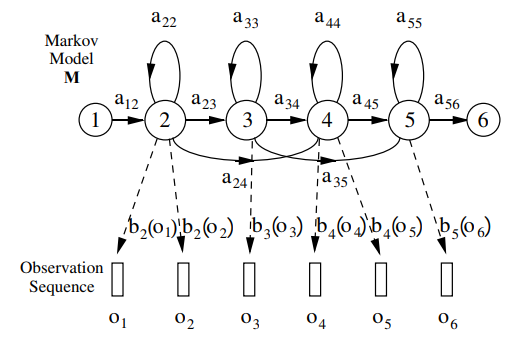
\includegraphics[width=9cm]{thesis/images/hmm}\\
  \caption{HMM Generative Model}\cite{young2002htk}\label{fig_2_1_hmm}
\end{figure}

In an HMM represented in figure \ref{fig_2_1_hmm} there are two important probabilities.  The first is the state transition probability given by $a_{ij}$ this is the probability to move from state $i$ to state $j$.  The second probability $b_j$ is the probability that an output probability when a state emits an observation.

Given that $X$ represents the sequence of states transitioned by a process a HMM the joint probability of $X$ and the output probabilities given the HMM is given as the following representation:
\begin{equation}P(\mathbf{O}|M)=\sum_Xa_{x(0)x(1)}\prod_{t=1}^Tb_{x(t)}(\mathbf{o}_t)a_{x(t)x(t+1)}
\label{eqn_2_4_hmm}
\end{equation}

Generally speaking, the HMM formulation presents 3 distinct challenges.  The first is that likelihood of a sequence of observations given in equation \ref{eqn_2_4_hmm} above.  The next two which we describe later is the inference and the learning problem.  While the inference problem determines the sequence of steps given the emission probabilities, the learning problem determines the HMM parameters, that is the initial transition and emission probabilities of the HMM model.

For the case of the inference problem, the sequence of states can be obtained by determining the sequence of states that maximises the probability of the output sequences.

\subsection{Challenges of Speech Recognition}
The realised symbol is assumed to have a one to one mapping with the segmented raw audio speech. However, the difficulty in computer speech recognition is the fact that there is significant amount of variation in speech that would make it practically intractable to establish a direct mapping from segmented raw speech audio to a sequence of static symbols. The phenomena known as co articulation has it that there are several different symbols having a mapping to a single waveform of speech in addition to several other varying factors including the speaker mood, gender, age, the medium of speech transduction, the room acoustics, et cetera.

Another challenge faced by automated speech recognisers is the fact that the boundaries of the words is not apparent from the raw speech waveform. A third problem that immediately arises from the second is the fact that the words from the speech may not strictly follow the words in the selected vocabulary database.  Such occurrence in speech recognition research is referred to as out of vocabulary (OOV) terms.  It is reasonable to approach these challenges using a divide and conquer strategy.  In this case, the first step in this case would be to create assumption that somehow word boundaries can be determined.  This first step in speech recognition is referred to as the isolated word recognition case.

\subsection{Challenges of low speech recognition}
Speech recognition for low resource languages poses another distinct set of challenges.  In chapter one, low resource languages were described to be languages lacking in resources required for adequate machine learning of models required for generative speech models.  These resources are described basically as a text corpus for language modelling, a phonetic dictionary and transcribed audio speech for acoustic modelling. Figure \ref{fig_2_2_asr_pipeline}, illustrates how resources of required for speech recognition are utilised.  It is observed that in addition to the three resources identified other processes are required for the speech decoder to function normally.  For example, aligned speech would also need to be segmented into speech utterances to ensure that the computer resources are used conservatively.

In terms of data collection processing \cite{besacier2014automatic} enumerates the  challenges for developing low resource ASR systems to include the fact that phonologies (or language sound systems) differ across languages, word segmentation problems, fuzzy grammatical structures, unwritten languages, lack of native speakers having technical skills and the multidisciplinary nature of ASR constitute impedance to ASR system building.

\begin{figure}
\centering
  % Requires \usepackage{graphicx}
  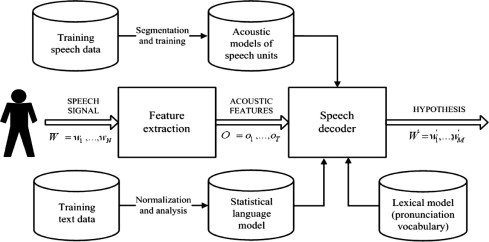
\includegraphics[width=10cm]{thesis/images/asr_pipeline}\\
  \caption{Automatic Speech Recognition Pipeline} \cite{besacier2014automatic}\label{fig_2_2_asr_pipeline}
\end{figure}

\section{Low Resource Speech Recognition}
In this system building speech recognition research, the focus was on the development of a language model and and an end-to-end speech model comparable in performance to state of the art speech recognition system consisting of an acoustic model and a language model.  Low resource language and acoustic modelling is now reviewed keeping in mind that little work has been done on low-resource end-to-end speech modelling when compared to general end-to-end speech modelling and general speech recognition as a whole.  

From an engineering perspective, a practical means of achieving low resource speech modeling from a language rich in resources is through various strategies of the machine learning sub-field of transfer learning.  

Transfer learning takes the inner representation of knowledge derived from a training an algorithm used from one domain and applying this knowledge in a similar domain having different set of system parameters. Early work of this nature was for speech recognition is demonstrated in \citep{vu2013multilingual} where multi-layer perceptrons were used to train multiple languages rich in linguistic resources. In a later section titled speech recognition on a budget, a transfer learning mechanism involving deep neural networks from \citep{kunze2017transfer} is described.

\subsection{Low Resource language modelling} \label{sec_lrlm}

General language modelling is reviewed and then Low resource language modelling is discussed in this section. Recall from the general speech model influenced by Bayes' theorem.  The speech recognition model is a product of an acoustic model (likelihood probability) and the language model (prior probability).  The development of  language models for speech recognition is discussed in \cite{juang2000automatic} and \cite{1996YoungA}. 

Language modelling formulate rules that predict linguistic events and can be modeled in terms discrete density $P(W)$, where  $W=(w_1, w_2,..., w_L)$ is a word sequence. The density function $P(W)$ assigns a probability to a particular word sequence $W$.  This value is determines how likely the word is to appear in an utterance. A sentence with words appearing in a grammatically correct manner is more likely to be spoken than a sentence with words mixed up in an ungrammatical manner, and, therefore, is assigned a higher probability. The order of words therefore reflect the language structure, rules, and convention in a probabilistic way. Statistical language modeling therefore, is an estimate for $P(W)$ from a given set of sentences, or corpus.

The prior probability of a word sequence $\mathbf{w}=w_1,\dots,w_k$ required in equation (2.2) is given by
\begin{equation}P(\mathbf{w})=\prod_{k=1}^KP(w_k|w_{k-1},\dots,w_1)
\label{eqn_c2_lm01}
\end{equation}

The N-gram model is formed by conditioning of the word history in equation \ref{eqn_c2_lm01}.  This therefore becomes
\begin{equation}P(\mathbf{w})=\prod_{k=1}^KP(w_k|w_{k-1},w_{k-2},\dots,w_{k-N+1})
\label{eqn_c2_lm02}
\end{equation}

N is typically in the range of 2-4.

N-gram probabilities are estimated from training corpus by counting N-gram occurrences.  This is plugged into maximum likelihood (ML) parameter estimate. For example, Given that N=3 then the probability that three words occurred is assuming $C(w_{k-2}w_{k-1}w_k)$ is the number of occurrences of the three words $C(w_{k-2}w_{k-1})$ is the count for $w_{k-2}w_{k-1}w_k$ then
\begin{equation}
P(w_k|w_{k-1},w_{k-2}\approx\frac{C(w_{k-2}w_{k-1}w_k}{C(w_{k-2}w_{k-1})}
\label{eqn_c2_lm03}
\end{equation}

The major problem with maximum likelihood estimation scheme is data sparsity. This can be tackled by a combination of smoothing techniques involving discounting and backing-off.  The alternative approach to robust language modelling is the so-called class based models \citep{Brown1992class,Kuhn1990cache} in which data sparsity is not so much an issue.  Given that for every word $w_k$, there is a corresponding class $c_k$, then,
\begin{equation}
P(\mathbf{w})\prod_{k=1}^KP(w_k|c_k)p(c_k|c_{k-1},\dots,c_{k-N+1})
\label{eqn_c2_lm04}
\end{equation}

In 2003,  \cite{bengio2003neural} proposed a language model based on neural multi-layer perceptrons (MLPs). These MLP language models resort to a distributed representation of all the words in the vocabulary such that the probability function of the word sequences is expressed in terms of these word-level vector representations. The result of the MLP-based language models was found to be, in cases for models with large parameters, performing better than the traditional n-gram models.

Improvements over the MLPs still using neural networks over the next decade include works of \cite{mikolov2011empirical,sutskever2014sequence,luong2013better}, involved the utilisation of deep neural networks for estimating word probabilities in a language model.  While a Multi-Layer Perceptron consists of a single hidden layer in addition to the input and output layers, a deep network in addition to having several hidden layers are characterised by complex structures that render the architecture beyond the basic feed forward nature where data flows from input to output hence in the RNN architecture we have some feedback neurons as well.  Furthermore, the probability distributions in these deep neural networks were either based upon word or sub-word models this time having representations which also conveyed some level of syntactic or morphological weights to aid in establishing word relationships.  These learned weights are referred to as token or unit embedding.

For the neural network implementations so far seen, a large amount of data is required due to the nature of words to have large vocabularies, even for medium-scale speech recognition applications.   \cite{kim2016character} on the other hand took a different approach to language modelling taking advantage of the long-term sequence memory of long-short-term memory cell recurrent neural network (LSTM-RNN) to rather model a language based on characters rather than on words.  This greatly reduced the number of parameters involved and therefore the complexity of implementation.  This method is particularly of interest to this article and forms the basis of the implementation described in this article due to the low resource constraints imposed when using a character-level language model.

Other low resource language modelling strategies employed for the purpose of speech recognition was demonstrated by \cite{xu2013cross}.  The language model developed in that work was based on phrase-level linguistic mapping from a high resource language to a low resource language using a probabilistic model implemented using a weighted finite state transducer (WFST). This method uses WFST rather than a neural network due to scarcity of training data required to develop a neural network. However, it did not gain from the high non linearity ability of a neural network model to discover hidden patterns in data, being a shallower machine learning architecture.

The method employed in this report uses a character-based Neural network language model that employs an LSTM network similar to that of \cite{kim2016character} on the Okrika language which is a low resource language bearing in mind that the character level network will reduce the number of parameters required for training just enough to develop a working language model for the purpose of speech recognition.  

\subsection{Low Resource Acoustic modelling}

Two transfer learning techniques for acoustic modelling investigated by \cite{povey2011subspace} and \cite{ghoshal2013multilingual} respectively are the sub-space Gaussian mixture models (SGMMs) and the use of pretrained hidden layers of a deep neural network trained multilingually as a means to initialise weights for an unknown language.  This second method has been informally referred to as the swap-hat method.

In an SGMM, emission densities of a hidden Markov Model (HMM) are modeled as mixtures of Gaussians, whose parameters are factorized into a globally-shared set that does not depend on the HMM states, and a state specific set.
The global parameters may be thought of as a model for the overall acoustic space, while the state-specific parameters provide the correspondence between different regions of the acoustic space and individual speech sounds.
The decoupling  of two aspects of speech modeling that makes SGMM suitable for different languages.

Sub-space Gaussian Mixture Models (SGMMs) has been shown to be suitable for cross-lingual modeling without explicit mapping between phone units in different languages.

Using layer wise pretraining of stacked Restricted Boltzmann Machines (RBMs) is shown to be insensitive to the choice of languages analogous to global parameters of SGMMs. Using a network whose output layer corresponds to context-dependent phone states of a language, by borrowing the hidden layers and fine-tune the network to a new language. The new outputs are scaled likelihood estimates for states of an HMM in a DNN-HMM recognition setup.
Used a 7-layer network without a bottleneck layer where the network outputs correspond to triphone states trained on MFCC features. Each layer contained about 2000 neurons.

\section{Groundwork for low resource end-to-end speech modelling}
The underpinning notion of this work is firstly a departure from the bottom-to-top baggage that comes as a bye-product of the generative process sponsored by the HMM-based speech models so that we can gain from simplifying the speech pipeline from acoustic, language and phonetic model to just a speech model that approximates the same process.  Secondly, the model developed seeks to overcome the data intensity barrier and was seen to achieve measurable results for GRU RNN language models.  Therefore adopting the same character-based strategy, this research performed experiments using the character-based bi-directional recurrent neural networks (BiRNN).  However, BiRNNs researchers have found them as other deep learning algorithms, as being very data intensive\cite{hannun2014deep}.  The next paragraphs introduce Deep-speech BiRNNs and the two strategies for tackling the data intensity drawback as related with low resource speech recognition.

\subsection{Deep speech}
Up until recently speech recognition research has been centred around improvements of the HMM-based acoustic models.  This has included a departure from generative training of HMM to discriminative training \citep{woodland2000large} and the use of neural network precursors to initialise the HMM parameters \citep{mohamed2012acoustic}.  Although these  discriminative models brought improvements over generative models, being HMM dependent speech models they lacked the end-to-end nature.  This means that they were subject to training of acoustic, language and phonetic models.  With the introduction of the Connectionist Temporal Classification (CTC) loss  function, \cite{graves2014towards} finally found a means to end-to-end speech recognition departing from HMM-based speech recognition. 

The architecture of the Deep-speech end-to-end speech recognition model \cite{hannun2014first} follows an end-to-end Bi-directional Recurrent Neural Network (BiRNN) and CTC loss function \citep{graves2006connectionist}.  The CTC loss function uses a modified beam search to sum over all possible input-output sequence alignments thereby maximising the likelihood of the output sequence characters.

\subsection{Speech Recognition on a low budget}

In this section, a recent transfer learning speech model model \citep{kunze2017transfer} that has some characteristics similar to the speech model developed in this thesis is reviewed.  The end-to-end speech model described by \cite{kunze2017transfer} is based on that developed by \cite{collobert2016wav2letter} and is based on deep convolutional neural networks rather than the Bi-RNN structure proposed by this work.  In addition it uses a loss function based on the AutoSegCriterion which is claimed to work competitively with raw audio waveform without any preprocessing.  The main strategy for low resource management in their system was the freezing of some layers within the convolutional network layer.  The low resource mechanisms used in this work includes the use of a unique scattering network being used as input features for the BiRNN model.  The fascinating similarity between the end-to-end BiRNN speech model developed in this work and the transfer learning model in \cite{kunze2017transfer} is the fact that the scattering network input are equivalent to the output of a light-weight convolutional neural network \cite{hannun2014first}.  Therefore the proposed system then approximates a combination of a recurrent neural network as well as a convolution neural network without the overhead of actually training a convolutional neural network (CNN).

Introduction of the unique scattering network is discussed in the next section.  It is worthy to note however that \cite{kunze2017transfer} uses a CNN network only while \citep{amodei2016deep} uses both RNN and CNN network.  The speech model in this thesis uses a BiRNN model in this work combines an RNN model with the scattering layer which represents a light-weight low resource friendly pseudo enhanced CNN backing.  What is meant by pseudo enhanced CNN backing is reserved for the next section, however, therefore, the proposed speech model in this speech model stands to gain from an enhanced but lightweight CNN combined with RNN learning.

\subsection{Adding a Scattering layer}

In machine learning, training accuracy is greatly improved through a process described as feature engineering.  In feature engineering, discriminating characteristics of the data is enhanced at the same time non-distinguishing features constituting noise is removed or attenuated to a barest minimum.  A lot of the components signal speech signal are due to noise in the environment as well as signal channel distortions such as losses due to conversion from audio signals to electrical signal in the recording system.

In figure \ref{fig_2_2_asr_pipeline}, feature engineering is done at the feature extraction stage of the ASR pipe line. It has be shown that a common technique using Mel-frequency cepstral coefficients (MFCCs) \citep{davis1990comparison} can represent speech in a stable fashion that approximate how the working of the human auditory speech processing and is able to filter useful components in the speech signal required for human speech hearing. Similar feature processing schemes have been developed include Perceptual Linear Prediction (PLP) \citep{hermansky1990perceptual} and RASTA \citep{hermansky1994rasta}. 

The scattering spectrum defines a locally translation invariant representation of a signal resistant to signal deformation over extended periods of time spanning seconds of the signal \citep{anden2014deep}. While Mel-frequency cepstral coefficients (MFCCs) are cosine transforms of Mel-frequency spectral coefficients (MFSCs), the scattering operator consists of a composite wavelet and modulus operation on input signals. 

Over a fixed time, MFSCs measure signal energy having constant Q bandwidth Mel-frequency intervals.  This procedure is susceptible to time-warping signal distortions since these information often reside in the high frequency regions discarded by Mel-frequency intervals.  As time-warping distortions isn't explicit classifier objective when developing these filters, there is no way to recover such information using current techniques. 

In addition, short time windows of about 20 ms are used in these feature extraction techniques since at this resolution speech signal is mostly locally stationary.  Again, this resolution adds to the loss of dynamic speech discriminating information on signal structures that are non-stationary at this time interval. To minimize this loss Delta-MFCC and Delta-Delta-MFCCs \citep{furui1986speaker} are some of the means developed to capture dynamic audio signal characterisation over  larger time scales.

By computing multi-scale co-occurrence coefficients from a wavelet-modulus operation \cite{anden2011multiscale} shows that non-stationary behavior lost by MFSC coefficients is captured by the scattering transform multi scale co-occurrence coefficients and the scattering representation includes MFSC-like measurements.  Together with higher-order co-occurrence coefficients, deep scattering spectrum coefficients represents audio signals similar to  models based on cascades of constant-Q filter banks and rectifiers.  In particular, second-order co-occurrence coefficients carry important  signal information capable of discriminating dynamic information lost to the MFCC analog over several seconds and therefore a more efficient discriminant than the MFCC representation. Second-order co-occurrence coefficients calculated by cascading wavelet filter banks and rectified using modulus operators have been evaluated as equivalent to a light-weight convolutional neural networks whose output posteriors are computed at each layer instead of only at the output layer \cite{mallat2016understanding}.

The premise for this work is that low speech recognition can be achieved by having higher resolution features for discrimination as well as using an end-to-end framework to replace some of the cumbersome and time-consuming hand-engineered domain knowledge required in the standard ASR pipeline.  In addition, this research work makes contributions to the requirements for the two tracks specified in the Zero Resource challenge of 2015 \citep{versteegh2015zero}.  The first requirement is sub-word modelling satisfied with using deep scattering network and the second that of spoken term discovery criteria being satisfied with the end-to-end speech model supplemented with a language model.

\section{Methodology}
System building methodology \citep{nunamaker1990systems} for speech recognition systems require models to be evaluated against speech recognition machine learning metrics.  For language models, perplexity metric was used for evaluation.  Bleu has also been used as a metric for evaluating language models.

Perplexity measures the complexity of a language that the language model is designed to represent \citep{1976jelinekcontinuous}. In practice, the entropy of a language with an N-gram language model $P_N(W)$ is measured from a set of sentences and is defined as
\begin{equation}H=\sum_{\mathbf{W}\in\Omega}P_N(\mathbf{W})
\label{eqn_c2_lm05}
\end{equation}

where $\Omega$ is a set of sentences of the language. The perplexity, which is interpreted as the average word-branching factor, is defined as
\begin{equation}B=2^H
\label{eqn_c2_lm06}
\end{equation}
\begin{equation}
PP(W)=P(w_1,w_2\dots w_N)^\frac{1}{N}
\label{eq6}
\end{equation}
\begin{equation}
PP(W)=\sqrt[N]{\prod_{i=1}^N\frac{1}{P(w_i|w_{i-1})}}
\label{eq7}
\end{equation}

Full speech recognition pipelines are usually evaluated against the Word Error Rate (WER).  WER is computed as follows:
\begin{equation}\label{eqn_2_3_wer}
WER=\frac{I+D+R}{WC}\times 100
\end{equation}

Metrics used for low speech recognition includes the ABX metric  \citep{versteegh2015zero}. Other common errors following a similar definition as the Word Error Rate (WER) are Character Error Rate (CER), Phoneme Error Rate (PER) and Syllabic Error Rate (SyER) and sentence error rate (SER).

\chapter{Recurrent Neural Networks in Speech Recognition}
The HMM model described in the Chapter \ref{c02} is uses the divide and conquer strategy which has been defined as a generative method in which we use the smaller components represented by the HMM to learn the entire speech process.   As also previously mentioned this is referred to as the bottom-up strategy.  The discriminative method however uses the opposite mechanism.  Rather than using the building blocks of speech to determine speech parameters of a HMM, the discriminative strategy determines the posterior probability directly using the joint probability distribution of the parameters involved in the discriminative process.  The discriminative parameters are discussed in this section where the Neural network discriminative approach is described beginning with the architecture.

\section{Neural network architecture}

The building block of a neural network simulates a combination of two consecutive linear and non-linear operations having many inputs interconnected with the linear portion of the network.  This rudimentary structure is described by McCullough and Pitts (1942) in  \cite{cowan1990discussion} as the Perceptron in figure \ref{fig_3_1_ptron} 

\begin{figure}
\centering
  % Requires \usepackage{graphicx}
  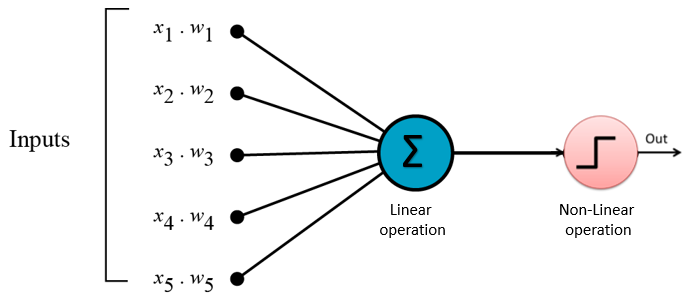
\includegraphics[width=7cm]{thesis/images/ptron2.png}\\
  \caption{Perceptron} \label{fig_3_1_ptron}
\end{figure}

The linear operation is the sum of the products of the input feature and a  weight vector set.  This vector sum of products is referred to as an affine transformation or operation.  The non linear operation is the given by any one of a selection of nonlinear functions.  In  figure \ref{fig_3_2_nn} this is shown as a step function.  The step function is activated (becomes 1) whenever the output of the linear function is above a certain threshold, otherwise remains at 0.  A simple neural network of perceptrons is formed by stacking the perceptrons into an interconnected layer as shown in the figure \ref{fig_3_2_nn}  :

\begin{figure}
\centering
  % Requires \usepackage{graphicx}
  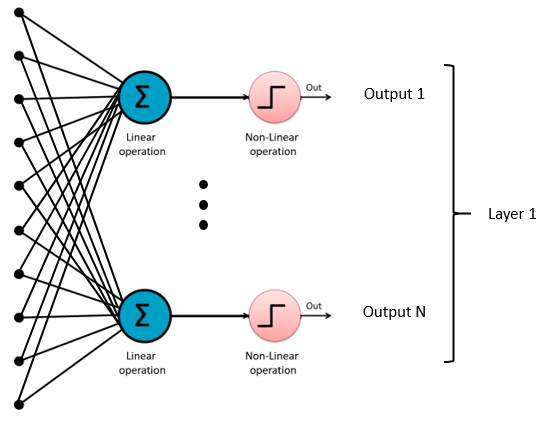
\includegraphics[width=7cm]{thesis/images/ptron3.png}\\
  \caption{Neural network} \label{fig_3_2_nn}
\end{figure}

In this regime each combination of linear operation followed by a non linear operation is called a neuron and the total number of neurons in the layer formed is termed as $M$-number of neurons in the layer.

\subsection{Multi-layer Perceptron (MLP)}
The multilayer Perceptron or MLP extends the basic Perceptron structure by adding one or more hidden layers.  These hidden layers comprise the outputs of one layer becoming the input of the next layer. In the simplest case having one hidden layer, the output of layer 1 becomes the input of the final output layer.  In comparison, the Perceptron is a one dimensional structure having one or more linear and non linear combination outputs, while the multilayer Perceptron is a 2-dimensional structure having one or more hidden layers of $N$ linear and non-linear combination outputs.  Mathematically speaking the output of each layer of an MLP having $N$ inputs and $M$ neurons is given by
\begin{equation}
z_j=h(b_j)=\frac{1}{ 1+e^{-b_j}} 
\label{eqn_c3_nn_01}
\end{equation}
 is the non-linear function while  is the linear function given by:
\begin{equation}
b_j=\sum_{i=0}^Nw_{ji}^{(1)}\qquad j=1,2,\dots,M
\label{eqn_c3_nn_02}
\end{equation}

For each layer in the MLP, the zeroth input value $x_0$ is 1 indicating a bias term.  This bias term is used in the neural network to ensure regularised and expected behaviour of the neural network.  In this example the non-linear step function is given by a more complex exponential.  In the next section the nonlinear functions for a multilayer Perceptron is derived.

\subsection{Sigmoid and soft-max Activation Function}
The combination of the linear function and the non linear function in the neural network could be said to be transformation of an algebraic problem to a probabilistic function.  In this case the "step" function is a squashing sigmoid-shaped function that converts the inputs into a Naive Bayes function evaluating the probability that an output belongs to any of the output classes $(C_y)$ given the data $(\mathbf{x})$.
\begin{equation}
p(C_1|\mathbf{x})=f(a)=f(\mathbf{w^\top x}+w_0)
\label{eqn_c3_nn_02}\end{equation}
In a two class problem with classes $C_1$ and $C_2$, the posterior probability of class $C_1$ is expressed using Bayes’s theorem
\begin{equation}
p(C_1|\mathbf{x})=\frac{p(\mathbf{x}|C_1)p(C_1)}{p(x|C_1)p(C_1)+p(\mathbf{x}|C_2)p(C_2)}
\label{eqn_c3_nn_03}\end{equation}
Dividing through by $p(\mathbf{x}|C_1)p(C_1)$ gives us
\begin{equation}
p(C_1|\mathbf(x)=\frac{1}{1+\frac{p(\mathbf{x}|C_1)p(C_1)}{p(\mathbf{x}|C_2)p(C_2)}}
\label{eqn_c3_nn_04}\end{equation}

If we define the ratio of the log posterior probabilities as
\begin{equation}
a=\ln\frac{p(\mathbf{x}|C_1)p(C_1)}{p(\mathbf{x}|C_2)p(C_2)}
\label{eqn_c3_nn_05}\end{equation}
If we substitute back into (4) we have:

\begin{equation}p(C_1|\mathbf{x})=f(a)=\frac{1}{1+e^{-a}}
\label{eqn_c3_nn_06}
\end{equation}

Here $a=\mathbf{w^\top x}=w_0$.  Thus the activation for the non-linear function is driven by the probability of the data to give the output class.  The probabilistic function here is called a sigmoid function due to the s-shaped graph that is plotted by the function.

Rather than using the sigmoid function for multi-class classification a similar soft max function is derived by using the log probability of classes. If $a_k=\ln(p(\mathbf{x}|C_k)p(C_k))$ then:
\begin{equation}
y_k=p(C_k|\mathbf{x})=\frac{e^{a_k}}{\Sigma_{\ell=1}^K e^{a_\ell}}
\label{eqn_c3_nn_07}\end{equation}
\begin{equation}
a_k=\sum_{i=0}^dw_{ki}x_i
\label{eqn_c3_nn_08}\end{equation}

Recall that in the generative classification method the problem is divided into sub problems by using the conditional probability, while in the discriminative approach the joint probability is determined by looking at the data directly.  This is what $p(C_k|\mathbf{x})$ represents.  However also, recall that we still need to determine the correct probability distribution represented by the data.  This is achieved by determining the values of the weights of the linear operation.  In the next section a method known as back propagation is discussed.  Back propagation is the training algorithm used to determine the weight vector of all the layers in the neural network.  Back propagation is an extension of the Gradient descent algorithm.

\subsection{Back propagation algorithm (backprop)}
In the previous section, the neural network architecture has been described as having $N$ inputs $M$ neurons and $L$ layers. Each layer comprises $M$ neurons of a maximum of $N$ inputs times $M$ neurons interconnections which embodies the inner product of the inputs and unknown set of weights. The output of this inner product is then passed to a logistic squashing function that results output probabilities.  The discriminative process is used here to determine the correct combination of weight vectors that accurately describe the training data.  For neural networks, the weight vectors at each layer are determined through propagating the errors back through each preceding layer and adjusting the weights according to the errors propagated each time a batch of the data is processed.  This process of continuously adjusting weights from back propagation continues until all the data is processed and a steady state has been reached.  The steady state refers to the fact that the error has reached a steady and/or acceptable negligible value.  This is often referred to in machine learning as convergence \citep{boden2002guide}.

\subsubsection{Gradient Descent}
The last section ended stating that the back-propagation algorithm is an extension of the gradient descent algorithm.  It has also been seen that back propagation works by propagating the error and making adjustments on the weights.  In this section, the Gradient Descent algorithm is reviewed and how it is used in back propagation is examined.  

The concept behind the Gradient descent algorithm is the fact that a function is optimized when the gradient of the function is equal to $0$.  Gradient descent algorithm is significant in machine learning applications because a cost function is easily defined for a particular machine learning application that is able to determine the error between the predicted value and the actual value.  Then, the parameters of the problem can be adjusted until the derivative of the cost function using gradient descent is zero.  Thus the machine learning algorithm adjusts its parameters until the error is minimised or removed.

A common error function or cost function for neural networks is the sum-of-squares error cost function.  This is obtained by summing the difference between the actual value and the machine learning model value over the training set $N$. 
\begin{equation}
E^n=\frac{1}{2}\sum_{k=1}^K(y_k^n-t_k^n)^2
\label{eqn_c3_nn_01}\end{equation}

In a neural network having a weight matrix $\mathbf{W}$ of $M$ neurons times $N$ inputs, the resulting gradient is a vector of partial derivatives of $E$ with respect to each element.  
\begin{equation}\nabla_{\mathbf{W}}E=\left(\frac{\partial E}{\partial w_{10}},\dots,\frac{\partial E}{\partial w_{ki}},\dots,\frac{\partial E}{\partial w_{Kd}}\right) 
\label{eqn_c3_nn_01}\end{equation}

The adjustment on each weight therefore on each iteration is:
\begin{equation}
w_{kj}^{\tau+1}=w_{kj}^{\tau}-\eta\frac{\partial E}{\partial w_{kj}}
\label{eqn_c3_nn_01}\end{equation}

Where $\tau$ is the iteration and $\eta$ is a constant learning rate which is a factor to speed up or slow down the rate rate of learning of the machine learning algorithm which in this case is the neural network.

\section{RNN, LSTM and GRU Networks}
Neural networks have become increasingly popular due to their ability to model non-linear system dynamics. Since their inception, there have been many modifications made to the original design of having linear affine transformations terminated with a nonlinear functions as the means to capture both linear and non-linear features of the target system. In particular, one of such neural network  modifications, namely the recurrent neural network, has been shown to overcome the limitation of varying lengths in the inputs and outputs of the classic feed-forward neural network.  In addition the RNN is not only able to learn non-linear features of a system but has also been shown to be effective at capturing the patterns in sequential data.  This section develops recurrent neural networks (RNNs) from a specialised multi-layer Perceptron (MLP) or the deep neural network (DNN).

\subsection{Deep Neural Networks (DNNs)}

Deep neural networks have been accepted to be networks having multiple layers and capable of hierarchical knowledge representation \citep{yu2016automatic}.
 This will therefore include multi-layer Perceptrons (MLPs) having more than one hidden layer \citep{dahl2012context} as well as deep belief networks (DBNs)\citep{mohamed2009deep,yu2010roles} having a similar structure.  Therefore, following the MLP architecture, A DNN uses multiple hidden layers and generates distribution function, $p(c|x_t)$ on the output layer when an input vector $\mathbf{x}_t$ is applied.  At the first hidden layer, activations are vectors evaluated using
\begin{equation}\mathbf{h}^{(1)}=\sigma(\mathbf{W}^{(1)T}\mathbf{x}_t+\mathbf{b}^{(1)})
\label{eqn_c3_dnn01}\end{equation}

The matrix $\mathbf{W}^{(1)}$ is the weight matrix and vector $b^{(1)}$, the bias vector for the layer.  The function $\sigma(\cdot)$ is the point-wise non-linear function.

DNNs activations  $$h^{(i)}$$ at layer i, at arbitrarily many hidden layers after the first hidden layer, are subsequently hidden activations are determined from

\begin{equation}\mathbf{h}^{(1)}=\sigma(\mathbf{W}^{(1)T}\mathbf{h}^{(i-1)}+\mathbf{b}^{(1)})
\label{eqn_c3_dnn02}\end{equation}

The distribution over all the possible set of characters $c$ is obtained in the final layer of the network in the exact way of a multi-layer Perceptron, that is, using soft max activation at the output layer of the form,
\begin{equation}p(c=c_k|x_t)=\frac{exp(-(\mathbf{W}^{(s)T}_kh^{(i-1)}+b_k^{(1)}))}{\sum_j exp(-(\mathbf{W}^{(s)T}_kh^{(i-1)}+b_k^{(1)}))}
\label{eqn_c3_dnn02}\end{equation}
$W_k^{(s)}$ and $b_k^{(k)}$ respectively are the output weight matrix and the scalar bias term of the $k$-th neuron. Accordingly, sub gradients for all parameters in the DNN are utilised to back propagate errors in weights during training for gradient-based optimisation techniques.  In DNN-HMM speech models,   DNNs are trained to predict probability distributions over senones.  However, in the model neural network described in section \ref{c3_ctc}, of this thesis, predicts per character conditional distributions.

Combining equations (\ref{eqn_c3_nn_01}, \ref{eqn_c3_dnn01}, \ref{eqn_c3_dnn02} and \ref{eqn_c3_dnn03}) the following simplified algorithm ensues

\begin{algorithm}[H]
\SetAlgoLined
\KwResult{Optimal weights }
 initialise weights randomly\;
 \While{error is significant or epochs less than maximum}{
  forward computation in equation (\ref{eqn_c3_dnn01} to \ref{eqn_c3_dnn03} )\;
  determine layer wise error for weights and biases $\Delta_\mathbf{W}E$ and  $\Delta_\mathbf{b}E$ \;
  update weights and biases according to gradient descent\;
 }
 \caption{DNN training algorithm}
\end{algorithm}

\subsection{Recurrent Neural Networks}
One of the two advantages RNNs have over regular DNNs is the ability to capture varying lengths of outputs to inputs.  That is for tasks such as language translation where there is no one to one correspondence of number of words in a sentence for example from the source language to the output destination language.  At the same time the sentence length appearing at the input and that appearing at the output differ for different sentences.  This is the first problem of varying lengths for input and output sequences.

The second issue that RNNs effectively contain as opposed to DNNs is capturing temporal relationships between the input sequences.  As was realised for hidden Markov models, it was seen that the HMM modeled not just observation likelihoods but also transition state likelihoods which were latent or hidden variables.  By tying the output of previous neuron activations to present neuron activations, a DNN inherits a cyclic architecture becoming a recurrent neural network (RNN). As a result, an RNN is to able capture previous hidden states and in the process derive memory-like capabilities \citep{yu2016automatic}.

In speech processing, it is observed that for a given utterance, there are various temporal dependencies which may not be sufficiently captured by DNN-based systems because DNN systems ignore previous hidden representations and output distributions at each time step $t$.  The DNN derives its output using only the  feature inputs $x_t$. The architecture of RNN to enable better modelling of temporal dependencies present in a speech is given in \citep{hannun2014first, yu2016automatic}. 

\begin{equation}h_t^{(j)}=\sigma(\mathbf{W}^{(j)T}h_t^{(i-1)}+\mathbf{W}^{(j)T}_kh_{t-1}^{(j)}+b^{(j)}))
\label{eqn_c3_rnn01}\end{equation}

It can be seen in equation (\ref{eqn_c3_rnn01}) above that given a selected RNN  hidden layer $j$, a temporally recurrent weight matrix $W^{(f)}$ is computed for output activations $h^{(j)}_{t-1}$ for the hidden activation vector of layer $j$ at time step $t - 1$ such that the output contributes to the standard DNN output of  $\mathbf{W}^{(j)T}h_t^{(i-1)}$. It can also be seen from  equation (\ref{eqn_c3_rnn01}) that the temporal recurrent weight matrix computation is a modified version of the standard DNN weight matrix computation and that the overall output is a superposition of the two.

Since computations for a RNN are the same as those described in standard DNN evaluations, it is possible to compute the sub gradient for  RNN architecture using the back propagation algorithm.  The modified algorithm appropriately called back propagation through time (BPTT) \citep{boden2002guide,jaeger2002tutorial} is derived as follows.  
\subsection{Back propagation through time (BPTT) algorithm}

First we define an arbitrary but carefully chosen number of time steps $t=1,2,\dots,T$ such that at each time step the states of the neuron activations $j=1,2,\dots,J$ are captured.
Using the sum-squared error as the cost function
\begin{equation}
E=c\sum_{t=1}^T||\mathbf{l}_t-\mathbf{y}_t||^2=c\sum_{t=1}^T\sum_{j=1}^L(l_t(j)-y_t(j))^2 \label{eqn_c3_bptt01}\end{equation}

Where $c$ is a gradient descent convenience factor, equation (\ref{eqn_c3_bptt01}). $||\mathbf{l}_t-\mathbf{y}_t||$ is the modulus of the difference between the actual output $\mathbf{y}_t$ and the label vector $\mathbf{y}_t$ at time $t$. The two-step BPTT algorithm described in \cite{yu2016automatic} is involves the recursive computation of the cost function and updating of the network weights.

For each of these steps recall from equation (\ref{eqn_c3_rnn01}) the activation of a hidden layer is a result of the composition of the regular DNN activation and an activation generated from weights from the previous time step.

The error term at final time t=T is
\begin{equation}
\delta^y_T(j)=-\frac{\delta E}{\delta y_T(j)}\frac{\delta y_T(j)}{\delta v_T(j)}=(l_T(j)-y_T(j))g'(v_T(j))\text{ for } j=1,2,\dots,L \label{eqn_c3_bptt04}\end{equation}
or
\begin{equation}
\mathbf{\delta}_T^y=(\mathbf{l}_T-\mathbf{y}_T)\bullet g'(\mathbf{v}_T) \label{eqn_c3_bptt05}\end{equation}
The error at the hidden layer is given as
\begin{equation}
\delta_T^h(j)=-\left(\sum_{i=1}^L\frac{\partial E}{\partial v_T(i)}\frac{\partial v_T(i)}{\partial h_T(j)}\frac{\partial h_T(j)}{\partial u_t(j)}\right)=\sum_{i=1}^L\delta_T^y(i)w_{hy}(i,j)f'(u_T(j))\text{ for } j=1,2,...,N \label{eqn_c3_bptt06}
\end{equation}
or $\delta_T^h=\mathbf{W}_{hy}^T\mathbf{\delta}_T^y\bullet f'(\mathbf{u}_T)$
where $\bullet$ is element-wise multiplication.

The recursive component for other time frames, $t=T-1, T-2, …, 1,$ the error term is determined as
\begin{equation}
\delta_t^y(j)=(l_t(j)-y_t(j))g'(v_t(j))\text{ for } j=1,2,\dots,L
\label{eqn_c3_bptt07}\end{equation}
or \begin{equation}
\mathbf{\delta}_t^y = (\mathbf{l}_t-\mathbf{y}_t)\bullet g'(\mathbf{v}_t) \label{eqn_c3_bptt08}\end{equation}

Therefore the output units are \begin{equation}\begin{aligned}\delta_t^h(j)&=-\left[\sum_{i=1}^N\frac{\partial E}{\partial\mathbf{u}_{t+1}(i)}\frac{\partial\mathbf{u}_{t+1}(i)}{\partial h_t(j)}+\sum_{i=1}^L\frac{\partial E}{\partial v_t(i)}\frac{\partial v_t(i)}{\partial h_t(j)}\right]\frac{\partial h_t(j)}{\partial u_t(j)}\\ &=\left[\sum_{i=1}^N\delta_{t+1}^h(i)w_{hh}(i,j)+\sum_{i=1}^L\delta_t^y(i)w_{hy}(i,j)\right]f'(u_t(j)) \text{ for }j=1,\dots,N \\ \text{ or } \delta_t^h&=\left[\mathbf{W}_{hh}^\top\mathbf{\delta}_{t+1}^h+\mathbf{W}_{hy}^\top\mathbf{\delta}_t^y\right]\bullet f'(\mathbf{u}_t)\end{aligned}\label{eqn_c3_bptt09}\end{equation}

Note that the error terms are propagated back from hidden layer at time frame $t + 1$ to the output at time frame $t$.

\subsubsection{Update of RNN Weights}
The weights are updated using the error terms determined in the previous section.  For the output weight matrices, we have \begin{equation}
\begin{aligned}w_{hy}^{new}(i,j)&=w_{hy}(i,j)-\gamma\sum_{t=1}^T\frac{\partial E}{\partial v_t(i)}\frac{\partial v_t(i)}{\partial w_{hy}(i,j)}=w_{hy}(i,j)-\gamma\sum_{i=1}^T\delta_t^y(i)h_t(j)\\ \text{ or }\mathbf{W}_{hy}^{new}&=\mathbf{W}_{hy}+\gamma\sum_{t=1}^T\mathbf{\delta}_y^t\mathbf{h}_t^\top\end{aligned} \label{eqn_c3_bptt10}\end{equation}
For the input weight matrices, we get \begin{equation}
w_{xh}^{new}(i,j)=w_{xh}(i,j)-\gamma\sum_{t=1}^T\frac{\partial E}{\partial u_t(i)}\frac{\partial u_t(i)}{\partial w_{xh}(i,j)}=w_{xh}(i,j)-\gamma\sum_{t=1}^T\delta_t^h(i)x_t(j) \label{eqn_c3_bptt11}\end{equation}
or \begin{equation}
\mathbf{W}_{xh}^{new}=\mathbf{W}_{xh}+\gamma\sum_{t=1}^T\mathbf{\delta}_h^t\mathbf{x}_t^\top \label{eqn_c3_bptt_13}\end{equation}
For the recurrent weight matrices we have 
\begin{equation} \begin{split}w_{hh}^{new}(i,j)&=w_{hh}(i,j)-\gamma\sum_{t=1}^T\frac{\partial E}{\partial u_t(i)}\frac{\partial u_t(i)}{\partial w_{hh}(i,j)}\\ &=w_{hh}(i,j)-\gamma\sum_{t=1}^T\mathbf{\delta}_h^t(i)h_{t-1}(j)\\ \text{ or }&=\mathbf{W}_{hh}^{new}=\mathbf{W}_{hh}+\gamma\sum_{t=1}^T\mathbf{\delta}_h^t\mathbf{h}_{t-1}^\top \end{split} \label{eqn_c3_bptt14}\end{equation}
In the BPTT algorithm the sub gradients are summed over all time frames. The algorithm is summarised below:

\begin{algorithm}[H]
\SetAlgoLined
\KwResult{Optimal weights }
 initialise weights randomly\;
 \For{error is significant or epochs less than maximum}{
  forward computation \;
  determine layer-wise error for weights and biases $\Delta_\mathbf{W}E$ and  $\Delta_\mathbf{b}E$ \;
  update weights and biases according to gradient descent\;
 }
 \caption{RNN training algorithm}
\end{algorithm}

\subsection{LSTMs and GRUs}

A special implementation of the RNN called the Long Short Term Memory (LSTM) has been designed to capture patterns over particularly long sequences of data and thus is an ideal candidate for generating character sequences while preserving syntactic language rules learned from the training data.

The internal structure and working  of the LSTM cell is documented by its creators in \cite{sak2014long}. The ability to recall information over extended sequences results from the internal gated structure which performs a series of element wise multiplications on the inputs and internal state of the LSTM cell at each time step.  In addition to the output neurons which in this text we refer to as the write gate and denote as the current cell state, $\mathbf{c}_t$, three additional gates (comprising a neural network sub-layer) located within the LSTM cell are the input gate, the forget gate and the output gate.  Together with the initial current state cell, these gates along with the current-state cell itself enable the LSTM cell architecture to store information, forward information, delete information and receive information.  Generally however, the LSTM cell looks like a regular feed-forward network having a set of neurons capped with a nonlinear function.  The recurrent nature of the network arises, however due to the fact that the internal state of the RNN cell is rerouted back as an input to the RNN cell or input to the next cell in the time-series giving rise to sequence memory within the LSTM architecture. Mathematically, these gates are formulated as follows:

\begin{equation}
\mathbf{i}_t=\sigma(\mathbf{W}^{(xi)}\mathbf{x}_t+\mathbf{W}^{(hi)}\mathbf{h}_{t-1}+\mathbf{W}^{(ci)}\mathbf{c}_{t-1}+\mathbf{b}^{(i)})
\label{eqn_c3_lstm01}
\end{equation}
\begin{equation}
\mathbf{f}_t=\sigma(\mathbf{W}^{(xf)}\mathbf{x}_t+\mathbf{W}^{(hf)}\mathbf{h}_{t-1}+\mathbf{W}^{(cf)}\mathbf{c}_{t-1}+\mathbf{b}^{(f)})
\label{eqn_c3_lstm02}
\end{equation}
\begin{equation}
\mathbf{c}_t=\mathbf{f}_t\bullet\mathbf{c}_{t- 1}+\mathbf{i}_t\bullet\tanh(\mathbf{W}^{(xc)}\mathbf{x}_t+\mathbf{W}^{(hc)}\mathbf{h}_{t-1}+\mathbf{b}^{(c)})\label{eqn_c3_lstm03}
\end{equation}
\begin{equation}
\mathbf{o}_t=\sigma(\mathbf{W}^{(xo)}\mathbf{x}_t+\mathbf{W}^{(ho)}\mathbf{h}_{t-1}+\mathbf{W}^{(co)}\mathbf{c}_{t-1}+\mathbf{b}^{(o)})\label{eqn_c3_lstm04}\end{equation}
\begin{equation}
\mathbf{h}_t=\mathbf{o}_t\bullet\tanh{(\mathbf{c}_t)}
\label{eqn_c3_lstm05}
\end{equation}

\begin{figure}
\centering
  % Requires \usepackage{graphicx}
  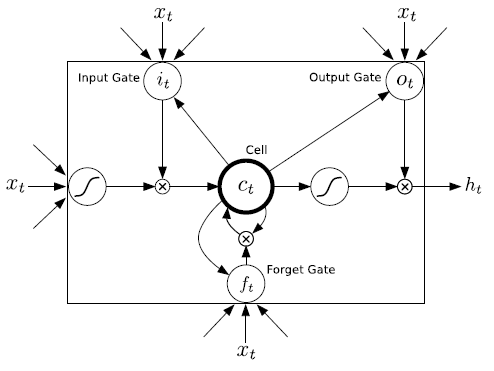
\includegraphics[width=7cm]{lstmcell}\\
  \caption{An LSTM Cell \cite{graves2013hybrid}}\label{fig_3_3_lstmcell}
\end{figure}

The gates in the above formula are illustrated in Figure \ref{fig_3_3_lstmcell}.  $\mathbf{i}_t$ represents the input gate, $\mathbf{f}_t$ is the forget gate and $\mathbf{o}_t$ represents the output gate.  At each of these gates therefore, the inputs consisting of hidden states in addition to the regular inputs are multiplied by a set of weights and passed through a soft-max function. These weights during training learn whether the gate will, during inference, open or not.  In summary, the input gate tells the LSTM whether or not to receive new information, the forget gate determines whether the current information it already has from the previous step should be kept or dropped and the output gate determines what should be forwarded to the next LSTM cell.  Note also that the LSTM has two sigmoid ($tanh$) activation functions utilised at the input and output of the current cell $\mathbf{c}_t$.

One particular variant of the original LSTM model is the GRU cell. Though simpler than an LSTM cell the GRU cell performs equally efficiently.  The main simplifications are that both state vectors are merged into a single vector $\mathbf{h}_{(t)}$. A single gate controller controls both the forget gate an the input gate.   If the gate controller outputs a 1, the input gate is open and the forget gate is closed.  If it outputs a 0, the opposite happens.  In other words, whenever a memory be stored, the location where it will be stored is erased first.  This is actually a frequent variant LSTM cell in and of itself. Finally, there is no output gate; the full vector cost is output at every time step.  However, there is a new gate controller that controls which part or the previous state will be shown to the main layer.

The overall architecture of a GRU is as follows:
\begin{equation}
\mathbf{z}_{(t)}=\sigma(\mathbf{W}_{xz}^T\cdot\mathbf{x}_{(t)}+\mathbf{W}_{hz}^T\cdot\mathbf{x}_{(t-1)})\label{eqn_c3_gru01}
\end{equation}
\begin{equation}
\mathbf{r}_{(t)}=\sigma(\mathbf{W}_{xr}^T\cdot\mathbf{x}_{(t)}+\mathbf{W}_{hr}^T\cdot\mathbf{x}_{(t-1)})\label{eqn_c3_gru01}
\end{equation}\begin{equation}
\mathbf{g}_{(t)}=\tanh(\mathbf{W}_{xg}^T\cdot\mathbf{x}_{(t)}+\mathbf{W}_{hg}^T\cdot(\mathbf{r}_{(t)}\otimes\mathbf{h}_{(t-1)}))\label{eqn_c3_gru01}
\end{equation}\begin{equation}
\mathbf{h}_{(t)}=(1-\mathbf{z}_{(t)})\otimes(\mathbf{h}_{(t-1)})+\mathbf{z}_{(t)}\otimes\mathbf{g}_{t}\label{eqn_c3_gru01}
\end{equation}

\section{Deep speech architecture}

This work makes use of an enhanced RNN architecture called the Bi-directional Recurrent Neural Network (BiRNN). While \cite{hannun2014first} assert that forward recurrent connections does reflect the sequential relationships of an audio waveform, perhaps the BiRNN model poses a more powerful sequence model.

The BiRNN is a preferred end to end mechanism due to the length of sequence over which temporal relationships can be captured.  This implies that BiRNNs will be suited for capturing temporal relationships over much longer sequences than a forward only RNN, because hidden state information is preserved in both forwards and backwards direction. 

In addition, such a model has a notion of complete sentence or utterance  integration, having information over the entire temporal extent of the input features when making each prediction. 

The formulation of the BiRNN is derived by starting off with the basic RNN architecture which is referred to as the forward architecture.  From the forward architecture we derive the backward architecture. If we choose a temporally recurrent layer $j$, the BiRNN forward and backward intermediate hidden representation $h^{(f)}_t$ and $h^{(b)}_t$ is given as. 
\begin{equation}h_t^{(f)}=\sigma(\mathbf{W}^{(j)T}h_t^{(i-1)}+\mathbf{W}^{(f)T}_kh_{t-1}^{(j)}+b^{(j)}))
\label{eqn_c3_ds01}\end{equation}
\begin{equation}h_t^{(b)}=\sigma(\mathbf{W}^{(j)T}h_t^{(i-1)}+\mathbf{W}^{(b)T}_kh_{t+1}^{(b)}+b^{(j)}))
\label{eqn_c3_ds02}\end{equation}

Temporal weight matrices $W^{(f)}$ and $W^{(b)}$ propagate $h^{(f)}_t$  and $h^{(b)}_t$ forward and backward in time respectively. 

\cite{hannun2014first} points out that the recurrent forward and backward components are evaluated entirely independent of each other and for optimal training, a modified non linearity function $\sigma(z) = min(max(z, 0), 20)$ is recommended. 

The final BiRNN representation $h^{(j)}_t$ for the layer is now the sum of the two RNN components,
 \begin{equation}h_t^{(j)}=h_t^{(f)}+h_t^{(b)}
\label{eqn_c3_ds03}\end{equation}
Also note that back propagation sub gradient evaluations is computed from the combined BiRNN structure directly during training.

\subsection{Connectionist Temporal Classification (CTC)}


\chapter{Deep Scattering network}
Curve fitting is a very common theme in pattern recognition. The concept of invariant functions convey mapping functions that approximate a discriminating function when a parent function is reduced from a high dimensional space to a low dimensional space \cite{mallat2016understanding}.  In this chapter an invariance function called a scattering transform  enables invariance of groups of deformations that could apply to speech signals thereby preserving higher level characterisations useful for classifying speech sounds. Works done by \citep{peddinti2014deep,zeghidour2016deep,anden2011multiscale,sainath2014deep} have shown that when the scattering spectrum are applied to speech signals and used as input to speech systems have state of the art performance.  In particular \cite{sainath2014deep} shows 4-7\% relative improvement in word error rates (WER) over Mel frequencies cepstral coefficients (MFCCs) for 50 and 430 hours of English Broadcast News speech corpus.  While experiments have been performed with hybrid HMM-DNN systems in the past, this thesis focuses on the use of scatter transforms in end-to-end RNN speech models.

This chapter iterates the use of the Fourier transform as the starting analysis function for building invariant functions and then discusses the Mel filter bank solution and then establishes why the scattering transform through the wavelet modulus operator provides better invariance features over the Mel filters.

\section{Fourier transform}
The Fourier transform often referred to as the power spectrum, allows us to discover frequencies contained within a function.  The Fourier transform is a convolution between a signal and a complex sinusoid from $-\infty$ to $+\infty$ (Figure \ref{fig_4_1_fourier_eqn}). 

\begin{figure}
\centering
  % Requires \usepackage{graphicx}
  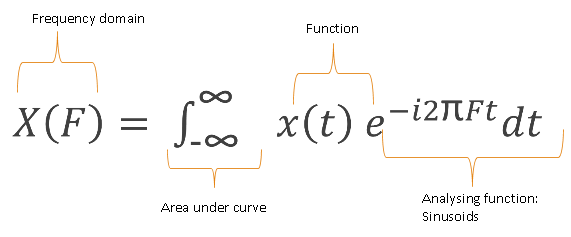
\includegraphics[width=7cm]{thesis/images/fourier.png}\\
  \caption{Fourier Equation} \label{fig_4_1_fourier_eqn}
\end{figure}
From the orthogonal property of complex exponential function, two functions are orthogonal if $\int f(x)g(x)=0$ where f(x) and g(x) are complimentary functions, one being referred to as the analysis equation and the other referred to as the synthesis function.

If the discrete form of the Fourier transform analysis equation is given by
\begin{equation}
a_k=\frac{1}{T}\int_{-T/2}^{T/2}x(t)e^{\left(-j\frac{2\pi kt}{T}\right)}
\label{eqn_c4_fourier01}
\end{equation}

Then, the corresponding synthesis equation is given by
\begin{equation}
x(t)=\sum_{k=-\infty}^{\infty}a_ke^{\left(j\frac{2\pi kt}{T}\right)}
\label{eqn_c4_fourier02}
\end{equation}

Recall that $x(t)$ is the original signal while $a_k$ is the Fourier Series coefficient.  This coefficient indicates the amplitude and phase of the original signal's higher order harmonics indexed by $k$ such that higher values of $k$ correspond to higher frequency components.  In a typical spectrogram (figure \ref{fig_4_2_spectral}), it can be seen that the energy of the signal is concentrated about a central region and then harmonic spikes of energy content exponentially decrease and taper off.  Therefore in figure \ref{fig_4_2_spectral}, the energies are concentrated at frequencies of about 100, 150 and 400 hertz.
\begin{figure}
\centering
  % Requires \usepackage{graphicx}
  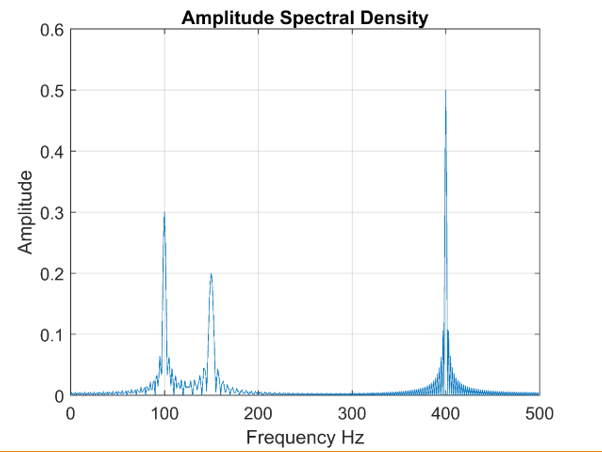
\includegraphics[width=7cm]{thesis/images/spectral.png}\\
  \caption{Sample Spectrogram} \cite{xxx}\label{fig_4_2_spectral}
\end{figure}

The Fourier transform discussed in the previous section constitutes a valuable tool for the analysis of the frequency component of a signal.  However is not able to determine when in time a frequency occurs hence is not able to analyse time related signal deformations.  The Short-time Fourier Transform (STFT) attempts to salvage this by windowing the signal in time signal and performing Fourier transforms over sliding windows sections of the original signal rather than the whole signal.  There is however, a resolution trade off that ensues from this operation such that, the higher the resolution in time accuracy, the lower the frequency accuracy and vice versa.  In the next section on the continuous wavelet transform, how the wavelet transform improves on the weaknesses of the Fourier Transform and the STFT is reviewed.

\section{Wavelet transform}
The continuous wavelet transform can be defined as a signal multiplied by scaled and shifted version of a wavelet function $\psi(t)$ referred to as the mother wavelet. The time-frequency tile-allocation of the three basic transforms examined in the first part of this chapter is illustrated in figure \ref{fig_4_3_tftile}

\begin{figure}
\centering
  % Requires \usepackage{graphicx}
  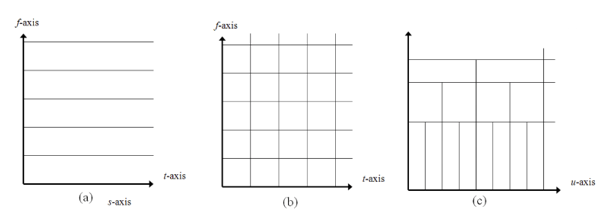
\includegraphics[width=14cm]{thesis/images/tftile}\\
  \caption{Time frequency tiling for (a) Fourier Transform (b) Short-time Fourier Transform (STFT) (c) Wavelet transform}\label{fig_4_2_tftile}
\end{figure}

It can be seen here that for the Fourier transform there is no time information obtained.  In the STFT, as there is no way of telling where in time the frequencies are contained, the STFT makes a blanket range of the resolution of the window and is therefore equally tiled potentially losing information based on this setup.  For the case of the wavelet, because it is a scaled and shifted convolution, it takes care of the this problem providing a good resolution in both time and frequency.  The fundamental representation of the continuous wavelet function is:
\begin{equation}
C(a,b)=\int f(t)\frac{1}{\sqrt{a}}\psi\left(\frac{t-b}{a}\right)dt\label{eqn_c4_wavelet01}
\end{equation}
In this equation, $a$ and $b$ respectively represent the scaling and shifting resolution variables of the wavelet function. This is referred to as a mother wavelet. A few other mother wavelet functions discussed later in this chapter. Generally a mother wavelet is identified as being energy spikes in an infinite signal whose accumulative energy sums to zero.

\section{Discrete and Fast wavelet transform}
Synthesis and analysis equations (\ref{eqn_c4_fourier02} and \ref{eqn_c4_fourier01}) can be formulated as a linear combination of the basis $\phi_k(t)$ such that the basis, $\phi_k(t)=e^{j2\pi kt}$, and it's conjugate or orthonormal basis, $\tilde{\phi}_k(t)=e^{-j2\pi kt}$, equations (\ref{eqn_c4_fourier02} and \ref{eqn_c4_fourier01}) now become

\begin{equation}
x(t)=\sum_{k}a_k\phi_k
\label{eqn_c4_dwt02}
\end{equation}

\begin{equation}
a_k=\int x(t)\tilde{\phi}_k(t)
\label{eqn_c4_dwt01}
\end{equation}

With respect to scaling and shifting variables of continuous wavelet transforms in equation (\ref{eqn_c4_wavelet01}), a similar linear combination transformation can be applied by constructing orthonormal bases parameters, referred to as scaling ($\phi$) and translating ($\psi$) functions. For example, a simple Haar mother wavelet transform associated with a delta function, it is seen that:
\begin{equation}
\phi_{j,k}(t)=2^{j/2}\phi(2^jt-k)
\label{eqn_c4_dwt03}
\end{equation}
\begin{equation}
\psi_{j,k}(t)=2^{j/2}\psi(2^jt-k)
\label{eqn_c4_dwt04}
\end{equation}
where j is associated with the dilation (scaling) parameter and k is associated with the position (shifting) parameter. If the Haar coefficients $h_{(\cdot)}[n]=\{1/\sqrt{2},1/\sqrt{2}\}$ are extracted we have the following dilation and position parameters.
\begin{equation}
\phi(t)=h_\phi[n]\sqrt{2}\phi(2t-n)
\label{eqn_c4_dwt05}
\end{equation}
\begin{equation}
\psi(t)=h_\phi[n]\sqrt{2}\psi(2t-n)
\label{eqn_c4_dwt06}
\end{equation}

For any signal, a discrete wavelet transform in $l^2(\mathbb{Z})^1$ can be approximated by
\begin{equation}
f[n]=\frac{1}{\sqrt{M}}\sum_kW_\phi[j_0,k]\phi_{j_0,k}[n]+\frac{1}{\sqrt{M}}\sum_{j=j_0}^\infty\sum_kW_\psi[j,k]\psi_{j,k}[n]
\label{eqn_c4_dwt07}
\end{equation}
Here $f[n],\phi_{j_0,k}[n]$ and $\psi_{j,k}[n]$ are discrete functions defined in [0,M - 1], totally M points.  Because the sets $\{\phi_{j_0,k}[n]\}_{k\in\mathbf{Z}}$ and $\{\psi_{(j,k)\in\mathbf{Z}^2,j\ge j_0}\}$ are orthogonal to each other.  We can simply take the inner product to obtain the wavelet coefficients.
\begin{equation}
W_\phi[j_0,k]=\frac{1}{\sqrt{M}}\sum_nf[n]\phi_{j_0,k}[n]
\label{eqn_c4_dwt08}
\end{equation}
\begin{equation}
W_\psi[j,k]=\frac{1}{\sqrt{M}}\sum_nf[n]\psi_{j,k}[n] \quad j\ge j_0
\label{eqn_c4_dwt09}
\end{equation}
Equation (\ref{eqn_c4_dwt08}) is called approximation coefficient while (\ref{eqn_c4_dwt09}) is called detailed coefficients.

These two components show that the approximation coefficient, $W_\psi[j_0,k]$, models a low pass filter and the detailed coefficient,$W_\psi[j_0,k]$, models a high pass filter. It is possible to determine the approximation and detailed coefficients without the scaling and dilating parameters. The resulting coefficients, called the fast wavelet transform, are a convolution between the wavelet coefficients and a down-sampled version of the next order coefficients.  The fast wavelet transform was first postulated in \citep{mallat1989theory}.
\begin{equation}
W_\phi[j,k]=h_\phi[-n]\ast W_\phi[j+1,n]|_{n=2k, k\ge 0}
\label{eqn_c4_dwt10}
\end{equation}
\begin{equation}
W_\psi[j_0,k]=h_\psi[-n]\ast W_\phi[j+1,n]|_{n=2k, k\ge 0}
\label{eqn_c4_dwt11}
\end{equation}

For analysis of the Haar wavelet and the derivation of equations (\ref{eqn_c4_dwt10} and \ref{eqn_c4_dwt11}) see appendix \ref{app01}.

\section{Mel filter banks}

Mel Frequency Cepstral Coefficients (MFCCs) are a feature widely used in automatic speech and speaker recognition. They were introduced by Davis and Mermelstein in the 1980's, and have been state-of-the-art ever since. Prior to the introduction of MFCCs, Linear Prediction Coefficients (LPCs) and Linear Prediction Cepstral Coefficients (LPCCs) and were the main feature type for automatic speech recognition (ASR), especially with HMM classifiers. 

An audio signal is constantly changing, so to simplify things we assume that on short time scales the audio signal doesn't change much (when we say it doesn't change, we mean statistically i.e. statistically stationary, obviously the samples are constantly changing on even short time scales). This is why we frame the signal into 20-40ms frames. If the frame is much shorter we don't have enough samples to get a reliable spectral estimate, if it is longer the signal changes too much throughout the frame.

The next step is to calculate the power spectrum of each frame. This is motivated by the human cochlea (an organ in the ear) which vibrates at different spots depending on the frequency of the incoming sounds. Depending on the location in the cochlea that vibrates (which wobbles small hairs), different nerves fire informing the brain that certain frequencies are present. Our periodogram estimate performs a similar job for us, identifying which frequencies are present in the frame.

The periodogram spectral estimate still contains a lot of information not required for Automatic Speech Recognition (ASR). In particular the cochlea can not discern the difference between two closely spaced frequencies. This effect becomes more pronounced as the frequencies increase. For this reason we take clumps of periodogram bins and sum them up to get an idea of how much energy exists in various frequency regions. This is performed by our Mel filter bank: the first filter is very narrow and gives an indication of how much energy exists near 0 Hertz. As the frequencies get higher our filters get wider as we become less concerned about variations. We are only interested in roughly how much energy occurs at each spot. The Mel scale tells us exactly how to space our filter banks and how wide to make them. 

Once we have the filter bank energies, we take the logarithm of them. This is also motivated by human hearing: we don't hear loudness on a linear scale. Generally to double the perceived volume of a sound we need to put 8 times as much energy into it. This means that large variations in energy may not sound all that different if the sound is loud to begin with. This compression operation makes our features match more closely what humans actually hear. Why the logarithm and not a cube root? The logarithm allows us to use cepstral mean subtraction, which is a channel normalisation technique.

The final step is to compute the DCT of the log filterbank energies. There are 2 main reasons this is performed. Because our filterbanks are all overlapping, the filterbank energies are quite correlated with each other. The DCT decorrelates the energies which means diagonal co-variance matrices can be used to model the features in e.g. a HMM classifier. But notice that only 12 of the 26 DCT coefficients are kept. This is because the higher DCT coefficients represent fast changes in the filterbank energies and it turns out that these fast changes actually degrade ASR performance, so we get a small improvement by dropping them.

\section{Deep scattering spectrum}
In this section reference is made to \citep{anden2011multiscale, anden2014deep, zeghidour2016deep}. For a signal $x$ we define the following transform $W_x$ as a convolution with a low-pass filter $\phi$ and higher frequency complex analytic wavelets $\psi_{\lambda_1}$:
\begin{equation}
Wx=(x\star\phi(t),x\star\psi_{\lambda_1}(t))_{t\in\mathbb{R},\lambda_1\in\Lambda_1} \label{eqn_c4_dss01}
\end{equation}

We apply a modulus operator to the wavelet coefficients to remove complex phase and extract envelopes at different resolutions
\begin{equation}
|W|x=\left(x\star\phi(t),|x\star\psi_{\lambda_1}(t)|\right)_{t\in\mathbb{R},\lambda_1\in\Lambda_1} \label{eqn_c4_dss02}
\end{equation}
$S_0x=x\star\phi(t)$ is locally invariant to translation thanks to the time averaging $\phi$.  This time-averaging loses the high frequency information, which is retrieved in the wavelet modulus coefficients $|x\star\psi_{\lambda_1}|$.  However, these wavelet modulus coefficients are not invariant to translation, and as for $S_0$, a local translation invariance is obtained by a time averaging which defines the first layer of scattering coefficients
\begin{equation}
S_1x(t,\psi_{\lambda_1})=|x \star\psi_{\lambda_1}| \star\phi(t)\label{eqn_c4_dss03})
\end{equation}
It is shown in \cite{anden2014deep} that if the wavelets $\psi_{\lambda_1}$ have the same frequency resolution as the standard Mel-filters, then the $S_1x$ coefficients approximate the Mel-filter coefficients.  Unlike the Mel-filter banks however, there is a strategy to recover the lost information, by passing the wavelet modulus coefficients  $|x\star\phi_{\lambda_1}|$ through a bank of higher frequency wavelets $\psi_{\lambda_2}$:
\begin{equation}
|W_2||x\star\phi_{\lambda_1}|=\left(|x\star\psi_{\lambda_1}|\star\phi,||x\star\psi_{\lambda_1}|\star\psi_{\lambda_2}|\right)_{\lambda_2\in\Lambda_2} \label{eqn_c4_dss04})\end{equation}
This second layer of wavelet modulus coefficients is still not invariant to translation, hence we average these coefficients with a low-pass filter $\phi$ to derive a second layer of of scattering coefficients.
 \begin{equation}
|W_2||x\star\phi_{\lambda_1}|=\left(|x\star\psi_{\lambda_1}|\star\phi,||x\star\psi_{\lambda_1}|\star\psi_{\lambda_2}|\right)_{\lambda_2\in\Lambda_2}\label{eqn_c4_dss04})\end{equation}

Repeating these successive steps of computing invariant features and retrieving lost information leads to the scattering spectrum, as seen in Fig. 1, however speech signals are almost entirely characterized by the first two layers of the spectrum, that is why a two layers spectrum is typically used for speech representation. It is shown in [6] that this representation is invariant to translations and stable to deformations, while keeping more information than the Mel-filter banks coefficients
\begin{figure}
\centering
  % Requires \usepackage{graphicx}
  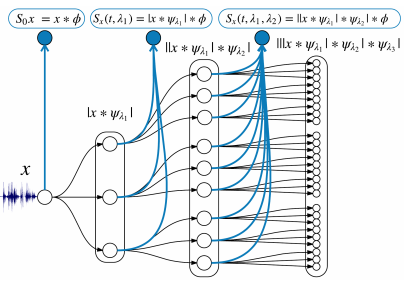
\includegraphics[width=7cm]{thesis/images/scatter.png}\\
  \caption{Scattering network - 2 layers deep} \cite{zeghidour2016deep}\label{fig_4_3_scatter}
\end{figure}


\spacing{1.0}
\bibliographystyle{plainnat}

\bibliography{bib}

\end{document}
